\documentclass[10pt,letterpaper,onecolumn,draftclsnofoot,journal]{IEEEtran}
\usepackage[margin=0.75in]{geometry}
\usepackage{listings}
\usepackage{color}
\usepackage{longtable}
\usepackage{graphicx}
\usepackage{caption}
\usepackage{float}
\usepackage{tabu}
\usepackage{enumitem}
\usepackage{courier}
\usepackage[hidelinks]{hyperref}

\setlength{\parindent}{0cm}
\setcounter{secnumdepth}{1}

\newcommand{\namesigdate}[2][6cm]{%
	\begin{tabular}{@{}p{#1}@{}}
		#2 \\[3\normalbaselineskip] \hrule \\[0pt]
		{\small \textit{Signature}} 
		\\[2\normalbaselineskip] \hrule \\[0pt]
		{\small \textit{Date}}
	\end{tabular}
}

\begin{document}
%\begin{titlepage}
%	\title{The ARLISS Project\\Progress Report\\Senior Capstone}
%	\author{Steven Silvers\\
%		Capstone Group 27\\Winter Term}
%	\date{\today}
%	\maketitle
%	\vspace{4cm}
%	\begin{abstract}
%		\noindent This document details Steven's experience working on the ARLISS Project during the winter term of 2017. This includes progress made, problems encountered and plans to address those problems as well as plans for future development of the project.
%	\end{abstract}

%\end{titlepage}
%\tableofcontents
%\clearpage

\title{The ARLISS Project\\Progress Report\\Senior Capstone}
\author{Steven Silvers\\
	Capstone Group 27\\Winter Term}
\date{\today}
\maketitle
\vspace{1cm}
\tableofcontents
\section{Introduction}
\par
This document covers the progress made by our team on the ARLISS Project over the course of winter term. The goal of this project is to work with a team of mechanical engineers and a team of electrical engineers to design and build a miniature rover that will be Oregon State University's entry into the annual ARLISS competition held in September. As part of the competition, the rover must be able to be deployed from a rocket at 10,000 feet AGL, land safely on the ground, unpack from any holding canister, lock on and autonomously drive to a finish destination at a set of provided GPS coordinates. Along the way the rover may encounter various obstacles that it will need to identify and avoid such as rocks or tire ruts.




\section{Weekly Summary of Winter Term}


\subsection{Week 1}
Start of winter term, over break I studied various autonomous driving methods since that is the main part of the project I am responsible for. I also looked at different hardware implementations and how they would possibly effect our programming decisions. We are communicating with the rest of the ARLISS capstone team to find a weekly meeting time, and have set our weekly TA meeting for Tuesdays at 1:30pm. Hopefully our whole team meeting time will be set soon so the ECE and ME teams can update us on their progress.

\subsection{Week 2}
Week two we met with our TA Franks for the first time this term, and discussed what is expected of the group as far as implementation of our project for this term. We as a group decided what a successful alpha version of our project would look like. We decided since the other two teams on our project would mostly likely not be finished with the hardware implementation until the end of the term, that for our alpha release we would write simulators for our individual modules to demonstrate that they function properly. The goal for the Beta release is to have the code implemented on hardware, but that is entirely dependent on the progress made by the ME and ECE groups.


\subsection{Week 3}
Week three we held a team wide meeting with the ECE and ME groups to better figure out time lines and what everyone is working on. It sounds like the ECE team has finally settled on using a Raspberry Pi zero as the main board for the rover, giving us a better idea of how we need to implement our code. The ME team told us that they will be designing and creating the wheel system in house so that it is fully customized to meet our needs. Progress has continued to be made on developing and simulating our individual code pieces in preparation for the week 6 alpha release.

\subsection{Week 4}
This week was mostly business as usual, we continued working on the alpha version of our project, as well as had an all group meeting that included our client Dr. Squires. My development module has been changed in that it will be getting a .mat file as input instead of a 2d binary array. This change will need to be reflected in the requirements document. As it is a late change, the alpha version will still be making use of a 2D binary array, and the plan is to change over to the .mat file for the beta version.

\subsection{Week 5}
Week five was spent doing work on the alpha version of the modules I am responsible for, mostly the obstacle avoidance system. Because of this modules' complexity it was decided that the alpha would be a lower level "prof of concept" and full functionality would be added by the 1.0 release. I edited both the tech review and the design document to reflect changes that had been made to the project for the sections I am responsible for. The biggest edit was for the control board, reflecting the decision made by the ECE team to use a Raspberry Pi Zero instead of one of the previously listed options.

\subsection{Week 6}
Week six was focused entirely on the upcoming alpha release and progress report. We decided that each team member would write their pieces individually and then combine them into one document Thursday, giving us plenty of time to submit the report on Friday. We got together with the ECE and ME teams for our weekly meeting, which ended early because all three groups were busy with progress reports and had nothing of significance to share. The ME team is uncertain of their capstone number, which hopefully they will figure out soon so that we can register as a group for Expo. The ME team also revealed to us during the short meeting that the rover frame did not hold up in testing and broke. They are now considering manufacturing the frame to the rover out of acrylic as it is a sturdy lightweight material that they believe will be easier to work with.

\subsection{Week 7}
Week seven I took a little bit of time to catch my breath and recover from being sick after a stressful week six. We are still waiting on the ME and ECE teams to figure out their capstone group numbers so that we can register for expo. The plan for week eight is to begin integrating our individual modules into a single system and to begin testing our system on the Raspberry Pi Zero.

\subsection{Week 8}
I spent most of this week attempting to merge my obstacle avoidance module with Zach's imaging module, with little to no success. I think what could be causing the problem is Zach and I may have OpenCV configured in different ways on our workstations, which is preventing me from properly compiling his source without making major changes. I will be sure to discuss with him in the coming days to see what we can do to fix this problem. Parts are still coming in for the ECE team, at the previous group meeting the servos had finally arrived that will be used for unpacking the rover from the payload once it lands. The ME team has a frame cut from acrylic, but is not yet assembled and last I heard from them they had not started on the wheel system yet. The plan currently is to have all of our modules working in a single system by the end of the term, and whether or not that gets implemented on hardware is Dependant on the progress made by the ECE and ME teams in the coming weeks.

\subsection{Week 9}
I made quite a bit of progress this week, I managed to successfully install Opencv on Linux, port Zach's imaging module so that it would run on Linux and not just from Visual Studio. I also added functionality so that it outputs a .csv file that I can easily open and use with my obstacle avoidance module. The .csv file contains values of zero where there is empty space(safe to drive) and nonzero and sometimes non integer values where there are edges. I just need to make a few edits to my module that allows it to adapt to the size of the .csv file, read any nonzero value as "1" and leave the zeros as they are, and it should be ready to check against real images.

\subsection{Week 10}
This week I finished combining the imaging and obstacle avoidance modules and began running tests of various images to make sure that the avoidance algorithm was reacting appropriately. Testing for this system will continue in spring term, as well as working on optimization as it currently takes a minute to run on a Raspberry Pi Zero which is too long for what we need. I know for certain there are a couple ways the code can be improved, there are a couple image filters being generated from testing that go unused, and a couple functions with multiple nested for loops can be merged into a single loop. I also laid the framework for the poster, as well as added information on my module to the poster. The only things still needed for the poster are a team photo, updated photos of the rover and of our image filters as well as a paragraph on Zach's imaging module.
\par
A change was made to how the .csv file is used, instead of taking in raw data from the picture it now only takes in 1's and 0's. This is possible due to OpenCV storing pictures using its own custom Mat data structure. My module now goes through this data structure pixel by pixel, checking the color values that are stored as type Vec3b. Since the filter makes the image black and white, its easy to store a 1 in the .csv file to correspond to a white pixel and a 0 to correspond to a black pixel. This approach made the summation in the obstacle avoidance module easier and more accurate.


\section{Modules I Am Responsible For}

\subsection{Control Board}
Progress for the control board module so far consists of coming together with the ECE and ME teams and selecting what board we would like to use for the project. At our first all group meeting we decided that a Raspberry Pi Zero would be the best fit for our project given the size constraints and the processing power needed by our imaging system. Once that decision was made, it was a matter of placing the order for the Pi Zero boards and updating the technology review and the design document to reflect the decision to use the Pi Zero.
\par
The Pi boards arrived shortly after the alpha version was turned in, the ECE team took two to work on building the electronics systems for the rovers while the CS team took one for testing our modules with. Paul held on to the board as he took up the task of doing most of the initial testing on it as well as installing Opencv and the Pi camera. At this point we are waiting on the ECE team to finish installing various sensors on the boards so that we can do testing with live data instead of just random testing with simulated values. We ran into a couple problems with the boards, namely we broke a camera port on one while trying to install the Pi camera. This problem was fixed by ordering a replacement board which arrived within the week. Another problem is that during weeks 9 and 10 the ECE group stopped communicating with either the CS or ME groups about progress and also stopped attending scheduled meetings and build days. This kept us in the dark about the progress of the hardware install by the ECE team on the Pi boards for multiple weeks, and we eventually ended up getting in contact with our client Dr. Squires about the problem, who was able to reach one ECE group member.
\begin{figure}[H]
	\centering
	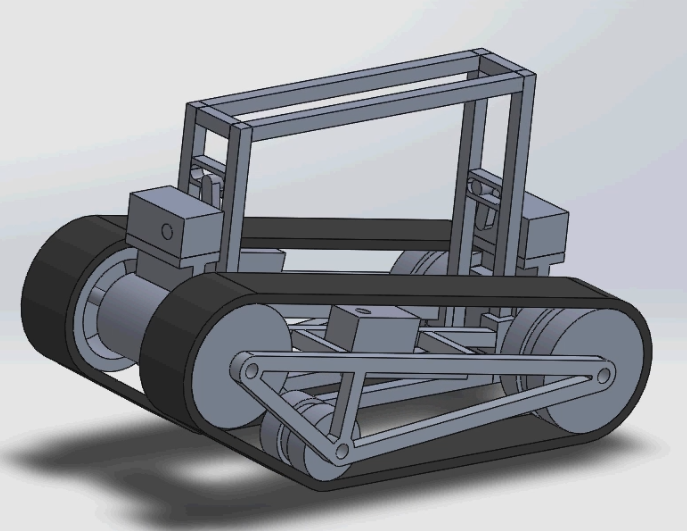
\includegraphics[scale = .4]{Capture.PNG}
	\caption{SolidWorks design of the rover}
	\label{fig:design}
\end{figure}
\subsection{Wheel System}
The wheel system for our rover will be designed and manufactured by our project's ME team here at Oregon State. As shown in figure \ref{fig:design}, our wheel system is a caterpillar track featuring three wheels per track, one of which is connected to a motor while the other two are for stabilization and guidance. Figure \ref{fig:rover} is the finished implementation of the wheel system for our rover, this photo was taken during our week 10 all team meeting. The wheel system was the last piece to get finished for the ME team apart from installing electronics into the rover, as they had to re-cut the caterpillar track to get a better fit. At this point it is safe to say that the wheel system module is complete and requires no further changes or development.

\begin{figure}[H]
	\centering
	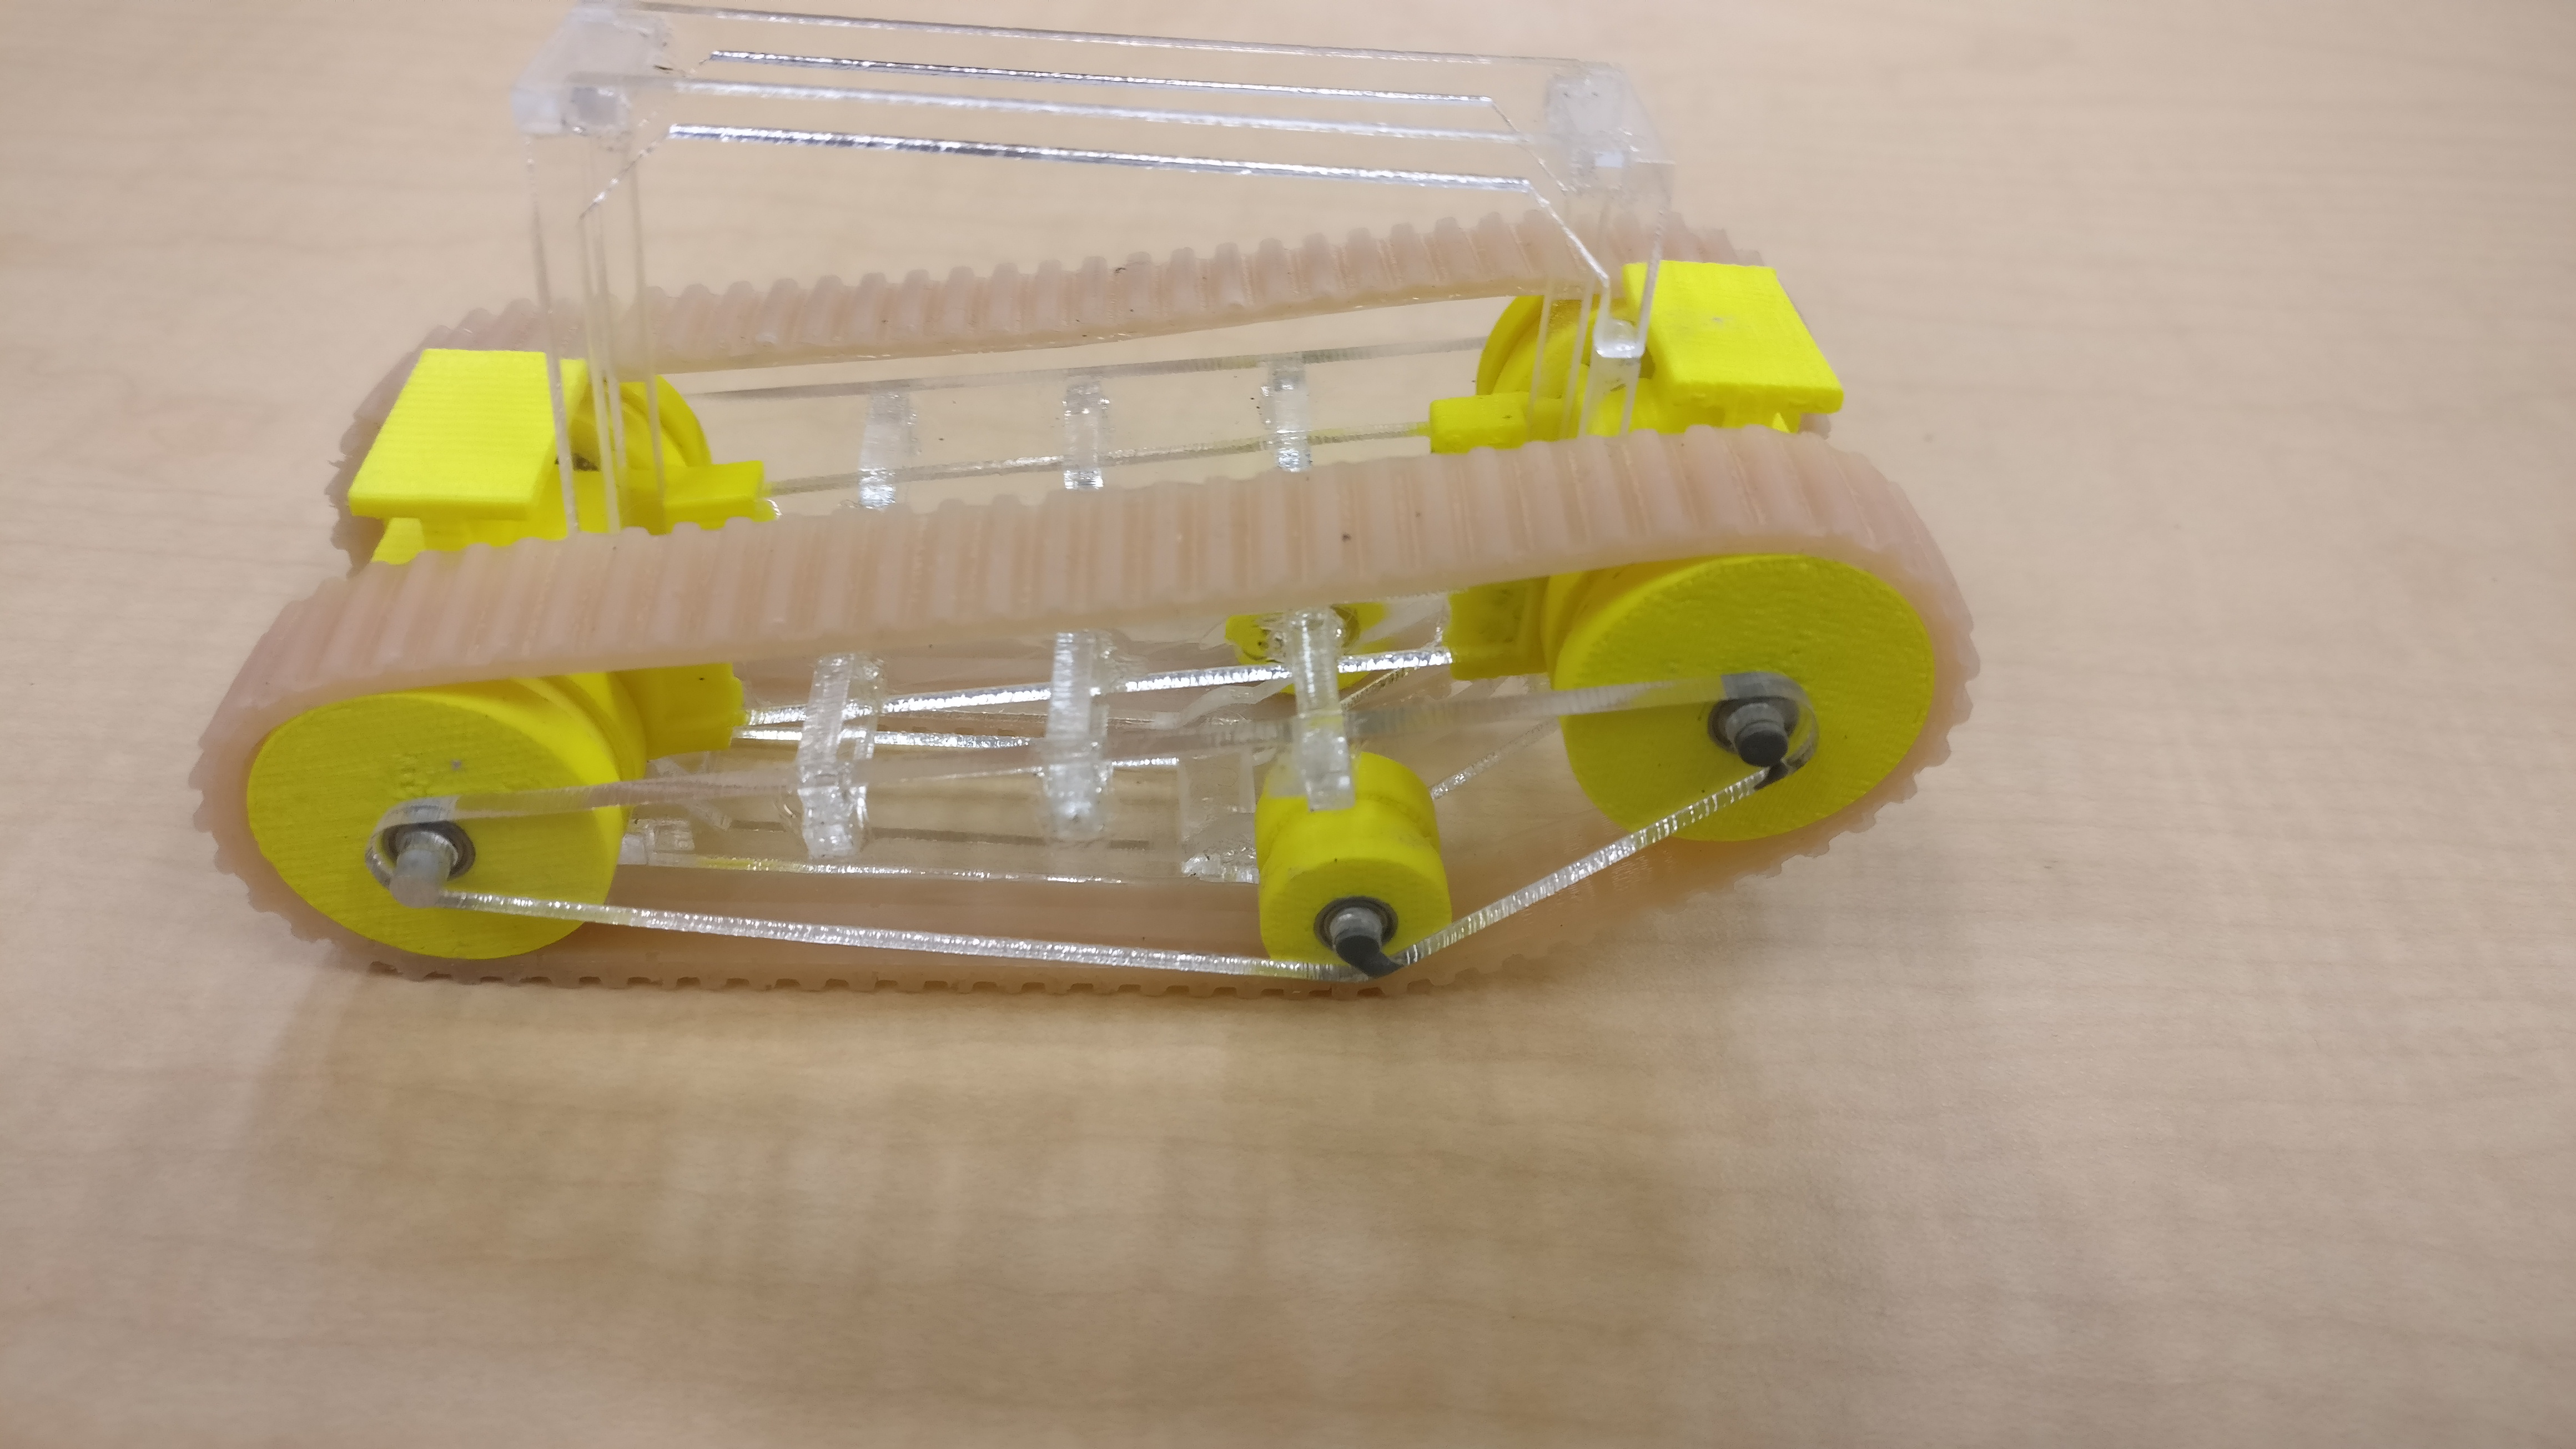
\includegraphics[scale = .05]{builtrover.jpg}
	\caption{Final wheel system}
	\label{fig:rover}
\end{figure}
\subsection{Obstacle Avoidance}
The obstacle avoidance system is what took up most of my time so far this term, as it is proving to be one of the trickier modules. I spent part of winter break as well as the first few weeks of winter term just focused on research for how to best implement a solution to this problem. The initial plan was to take in a 2D binary array as input from the imaging module developed by Zach where ones represent edges detected in an image, and zeros are unchanging terrain.
\begin{figure}[H]
	\centering
	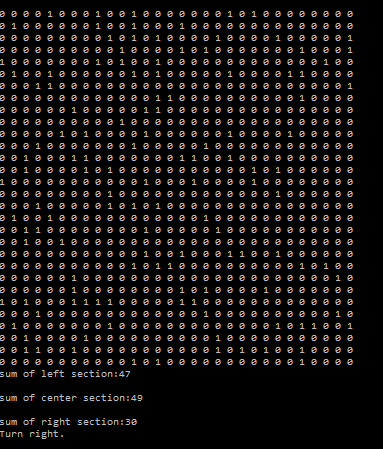
\includegraphics[scale = .75]{obstacleavoidance.png}
	\caption{output from alpha version}
	\label{fig:obstacle}
\end{figure}
\par
The original obstacle avoidance algorithm would splits the array into three large columns, left, center and right, and then sums those columns. This summation tells us where the most edges are, which translates to where the roughest terrain is. In figure \ref{fig:obstacle} it shows that the sum of the right column was the lowest, so the rover should turn right to avoid the rougher terrain in front of it and to the left. For testing purposes, the array used in the alpha release is randomly populated with ones and zeros. The current plan is for the beta version to be tested with actual images to ensure accuracy and logical correctness of the algorithm.
\begin{figure}[H]
	\centering
	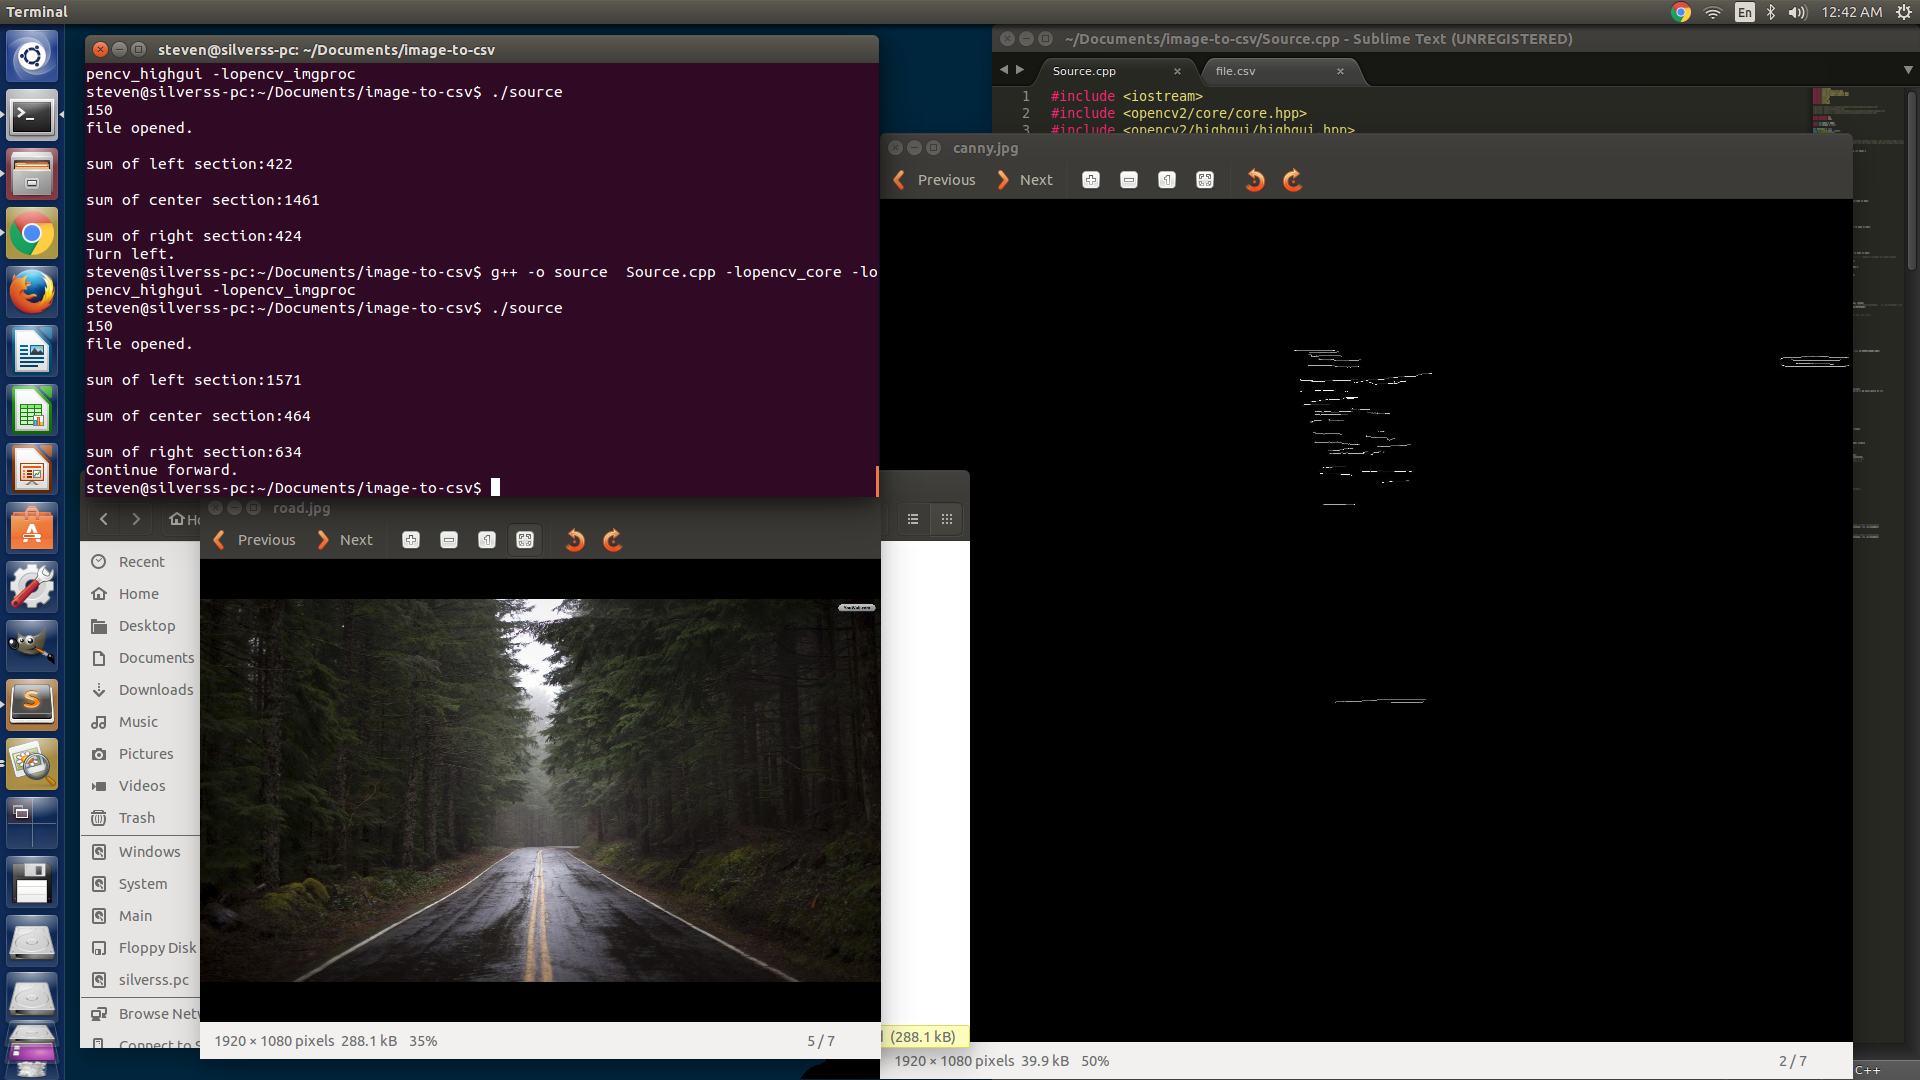
\includegraphics[scale = .25]{demo.png}
	\caption{output from beta version}
	\label{fig:beta}
\end{figure}
\par
Currently the obstacle avoidance module has been successfully combined with the imaging module and ran on the Raspberry Pi Zero. This means it currently can take a hard-coded image file, filter the image using OpenCV, determine which of the three sections of the image has the fewest edges and then turn that direction. As seen in figure \ref{fig:beta}, the program takes in the photo of the forest road, puts it through a filter to find the edges and then gives an output stating which direction should be traveled, in this case it said to continue straight down the road. One major problem came up while testing on the Raspberry Pi, which is it would take almost a minute for this module to go from a picture to giving a direction. We want this time to be much lower, and we plan to lower this time with a few optimizations. First we will use a lower resolution image in the implementation, the current test images are 1080p which is much more detail than we need. We will then strip out a few filters that were only used during testing but don't actually contribute to the implementation. If further optimization is needed, there are multiple nested loops that perform somewhat redundant tasks that could potentially merged into a single nested loop. Apart from fixing these problems, the plan is to switch the module over to take in images from the Pi camera instead of hard-coded file names, and to adjust testing constants to adjust with the new file dimensions as they come in from the camera.

\section{A Reflection of Development Period}
\begin{tabular}{ |p{0.3\linewidth}|p{0.3\linewidth}|p{0.3\linewidth}|  }
	\hline
	\multicolumn{3}{|c|}{Retrospective} \\
	\hline
	Positives& Deltas &Actions \\
	\hline
	Our group continues to work together and communicate well. &
	Make wiki pages on time.&
	Send each other reminders to do the wiki pages on Friday. \\
	
	Almost all software modules have been finished. &
	Github repo is becoming cluttered and messy &
	Reorganize repo to make docs easier to find, remove unnecessary files \\
	
	We shouldn't have much work to do during spring term &
	Haven't tested code on hardware yet & Communicate with ECE team to find out when it will be ready.  \\
	\hline
\end{tabular}

\vspace{1cm}
\par
We had a very successful term for implementation of our project. I believe Zach is still working on developing  machine learning for the finding the end cone module. Other than that the rest of the software modules are either in a fine tuning and testing stage or are waiting for the ECE team to finish the hardware drivers so that we can begin running tests on the hardware to ensure everything works properly. I am happy with what we as a team have produced for this end of winter term beta release.

\section{Team Review}
\subsection{Paul Minner}
Paul and I shared a lot of the management load, both of us communicating with the other groups in our team and by setting plans for finishing assignments. Paul represented our group at a few of the rover build days, as well as took on the role of combining all of our modules into a single system. Paul also took care of setting up and installing software on the Raspberry Pi Zero, and tested our modules on it. I believe Paul had a higher contribution to the project than the rest of the group, as he took on extra responsibilities such as integrating the modules and setting up the Pi, as well as showing up and representing the CS team at build days.

\subsection{Zhaolong Wu}
Zhaolong attended build days as another representative of the CS group, and also managed the task of tracking down our client to get signatures on our various documents. He finished his modules he was responsible for on time. Zhaolong made an average contribution to the group, always communicated with the team when needed and made an overall positive impact on the project.
\subsection{Zachary DeVita}
Zach worked a lot this term on developing a machine learning system for our rover so that it could find the finish pole through object identification instead of blindly looking for it. Unfortunately, some of the other modules he was working on took a back seat to this and I ended up finishing the imaging module. While taking up the task of machine learning was huge and may be a better way to find the finish pole than our original plan, it may have been a bit more than what was needed for our project. I would say that Zach made an average contribution to our project.
\subsection{Steven Silvers}
Apart from completing my modules on time as well as one of Zach's, I also took on editing our video presentations, setting up a web space for our project submissions and setting up our Expo poster so that our group can add information easily. As mentioned previously, I shared the management role with Paul, communicating with other teams in our group quickly and making sure our group is in a position to turn in our reports and presentations on time. Due to finishing other group members modules and setting up and managing the non-coding assignments I would rate my contribution at average to slightly above average.
\subsection{Team as a Whole}
I would say we work quite well as a development team, we have our hiccups here and there but overall we get our work done, communicate well and make all of our deadlines. Compared to how I've seen other groups interact in the capstone lab, we are doing very well working together and I'm very happy with our group.

\section{Conclusion}
I would rate this term overall as a success for our development team, We are in position to finish our project early spring term without having to scramble to finish in time for expo. The only step that remains is to implement our code on the rover hardware, which we are ready to start doing as soon as the ECE team has the hardware finished an installed in the rover. There is potential for problems to arise spring term, mostly that we aren't entirely sure what the finished hardware implementation will look like or how our code will need to be adapted to work with it, but I believe that we should be able to overcome any unforeseen obstacles that we come across.
\clearpage

\pagenumbering{gobble}
\vspace{1in}

\end{document}
